\documentclass[a4paper]{article}
\usepackage{graphics}
\usepackage{epsfig}
\usepackage{graphicx}
\usepackage{sverb}
\usepackage{verbatim}
\usepackage{url}
\usepackage{float}
\usepackage{fancyhdr}
\usepackage[utf8]{inputenc}

\pagestyle{fancy}
\fancyhead{}
\fancyfoot{}
\fancyfoot[CO,CE]{Author: Robert Foss - 8707174051 \\ \thepage}
\renewcommand{\headrulewidth}{0pt}
\title{Project 1\\ FMN011}
\author{Robert Foss (dt08rf1@student.lth.se)}
\date{} % Blir dagens datum om det utelmnas

\begin{document} % Br�jan p dokumentet
\maketitle
\thispagestyle{empty}
\newpage
\tableofcontents
\thispagestyle{empty}
\newpage

% \begin{EPIC TEXT}



\section{Introduction}
Newton's law of cooling is not solvable algebraically, due to it being a nonlinear equation,  however it possible to produce a solution analytically.

The aim of this project is to analytically calculate a solution for Newton's law of cooling.

\begin{comment}Briefly describe the general problem you want to solve and why a numerical or computational solution (as opposed to an exclusively analytical solution) is required.
\end{comment}

\subsection{Problem background}
The issue lies in determining the time of death for professor Sommar and thereby confirming the alibi of instructor T�gersson.

\section{Numerical Considerations}
Implementations of the following methods were created; Bisection, Secant root, Fixed point iteration and Newton-Raphson's method.
Matlab and Ocatave\cite{octave} was the only software directly used. Specific matlab functions used include; fzero (control), anonymous functions, fplot, plot, vectors, sym, feval, inline, diff, xlabel, ylabel, title and plot.
\begin{comment}
Briefly discuss the specific methods, software or algorithms you selected for this problem. Mention any specific features of MATLAB you exploited.
\end{comment}

\section{Results}
\subsection{Task 1}
$T' = -k(T - T_{office}) = -k(T-(22+0,5t)) \leftrightarrow T' + kT = -k(22+0,5t)$
\\
\\
Integrating factor produces:
\\
$T = e^{-kt} k (\int{22 e^{kt} dt} + \int{\frac{t}{2} e^{kt} dt}) + c e^{-kt}$
\\
$= e^{-kt}  k  ([\frac{22}{k}e^{kt}] + ([\frac{e^{kt}}{2k}] - \int{\frac{e^{kt}}{2k} dt})) + c e^{-kt}$
\\
$=22+0.5t-\frac{1}{2k} + c e^{-kt}

\subsection{Task 2}
$T(0) = 32$, given in the story of the problem.
\\
$T(0) \leftrightarrow 22 - \frac{1}{2k}+c = 32 \leftrightarrow c = (10 - \frac{1}{2k})$
\\
$T(1) = 29$, given in the story of the problem.
\\
$T(1) \leftrightarrow 22,5 - \frac{1}{2k}ce^{-k} \leftrightarrow c = (7 + \frac{1}{2k})e^{k}$
\\
$\leftrightarrow 7+\frac{1}{2k} = (10-\frac{1}{2k})e^{-k}$

\subsection{Task 3}
\label{task3}
The bisection method is an iterative method which repeatedly selects a subinterval where the root can found.

The choices of a and b were based on the criteria that $f(a)$ and $f(b)$ have opposite signs.
A and b were chosen after a $f(k)$ was plotted for roots in the interval $[0,10]$, as can be seen in Appendix B, section \ref{froot}. The tolerance was chosen according to definition 1.3\cite{kursbok}, $\frac{10^{-p}}{2}$. Where $p$ is the number of significant digits. Nmax was chosen any way that won't limit the precision of the function. e was chosen to produce 6 significant digits. The function used can found in Appendix A, section \ref{bisection}.
\begin{verbatim}
format long;
f=@(k)(10+1/(2*k))*exp(-k)-7-1/(2*k);
a=0.1;
b=1;
e=0.5*10^(-2);
Nmax=99;
[answer, iterations, err_qoutient, err] = bisection(f,a,b,e,Nmax);
answer = 0.2898
\end{verbatim}

\subsection{Task 4}
The secant root method is an iterative method which assumes a function is approximately linear in an interval and iteratively approximates the root of secant.

The choices of p0 and p1 are due to them being near the solution, as indicated by Task 3. The tolerance $s=e=10^{-7}$ was chosen to only tolerate errors smaller than the precision desired. Nmax was chosen in a way that won't limit the precision of the function. The function used can found in Appendix A, section \ref{secantroot}.
\begin{verbatim}
format long;
f=@(k)(10+1/(2*k))*exp(-k)-7-1/(2*k);
p0=0.1;
p1=1;
s=10^-7;
e=10^-7;
Nmax=99;
[answer, iterations, err_qoutient, err] = secantroot(f,a,b,s,e,Nmax);
answer = 0.296703053360269
\end{verbatim}

\subsection{Task 5}
The fixed point method is a method for iteratively finding a $x = f(x)$.

$g(x)= x$ was calculated and found to be $g(k)= k = log(\frac{10+\frac{1}{2k}}{7+\frac{1}{2k}})$. x0 was chosen due to it being near the solution, as indicated by Task 4. The tolerance $e=10^{-7}$ was chosen to only tolerate errors smaller than the precision desired. Nmax was chosen in a way that won't limit the precision of the function. The function used can found in Appendix A, section \ref{fixedpoint}.
\begin{verbatim}
format long;
g=@(k)log((10+1/(2*k))/(7+1/(2*k)));
x0=1;
e=10^-7;
Nmax=99;
[answer, iterations, err_qoutient, err] = fixedpoint(g,x0,e,Nmax);
answer = 0.296703056932817
\end{verbatim}

\subsection{Task 6}
Newton-Raphson's method is an iterative method that utilizes the first terms of the Taylor series for $f(x)$

x0 was chosen due to it being near the solution, as indicated by Task 4. The tolerance $e=10^{-7}$ was chosen to only tolerate errors smaller than the precisionv desired. Nmax was chosen in a way that won't limit the precision of the function. The function used can found in Appendix A, section \ref{newton}.

\begin{verbatim}
format long;
f=@(k)log((10+1/(2*k))/(7+1/(2*k)));
x0=1;
e=10^-7;
Nmax=99;
[answer, iterations, err_qoutient, err] = newton(f,x0,e,Nmax);
answer = 0.296703053214996
\end{verbatim}

$k=0.296703$ will be used for the approximation of $t_{d}(t) = 22 - 37 \frac{t}{2} -\frac{1}{2k} + (10 + \frac{1}{2k})e^{-kt}$. x0 was chosen as the professor has been dead for atleast 0 hours. The tolerance, e, was chosen to provide a solution with minimal residual. Nmax was chosen in a way that won't limit the precision of the function.
\begin{verbatim}
format long;
f= @(t)22-37+t/2-1/(2*0.296703)+(10+1/(2*0.296703))*exp(-0.296703*t)
x0=0
e=10^-70;
Nmax=99;
[answer, iterations, err_qoutient, err] = newton(f,x0,e,Nmax);
answer = -1.332487352900656
\end{verbatim}
Meaning that the professor died approximately 1.33 hours earlier than $T(0)$, about 6:40 p.m.

\subsection{Task 7}
9 significant digits were chosen. Leading to a tolerance of $10^{-10}$ for every method except for the bisection method, which's tolerance was set $\frac{10^{-9}}{2}$ in accordance with def. 1.3\cite{kursbok}. The points for the bisection method and the secant root method were chosen to be $-2$ and $0$, based on the root plot for $T(t)$ found in Appendix B, section \ref{troot}. x0 for Newton-Raphson and the fixed point iteration method was chosen be $-1$, based the previously mentioned root plot for $T(t)$. Nmax was selected to a large number, $Nmax=999$, to keep it from interfering. The function being approximated was once again $t_{d}(t) = 22 - 37 \frac{t}{2} -\frac{1}{2k} + (10 + \frac{1}{2k})e^{-kt}$, with $k=0.29670$ in accordance with Task 6. $g_{d}(t) = t = \frac{log(22-37+\frac{t}{2}-\frac{1}{2k})}{log(10+\frac{1}{2k})k}$ was used for the fixed point iteration method.

\\
\resizebox{\textwidth}{!}{%
\begin{tabular}{llll}
\\
Root finding method & Error & Iterations & Convergence speed, last iter. \\ \hline
Bisection method$^{[\ref{bisection}]}$ & $1.1642*10^{-10}$ & $34$ & $0.5$ \\
Secant root method$^{[\ref{secantroot}]}$ & $8.2710*10^{-10}$ & $6$ & $0.0002$ \\
Fixed point iteration$^{[\ref{fixedpoint}]}$ & $1.1818*10^{-10}$ & $9$ & $0.0458$ \\
Newton-Raphson's method$^{[\ref{newton}]}$ & $0$ & $4$ & $0$ \\
\end{tabular}}

\section{Analysis}
Error quotient plots can be found in Appendix: C, section \ref{appc}. Bisection$^{[\ref{qbisect}]}$ and fixed point iteration$^{[\ref{qfixedpoint}]}$ are shown to have a linear convergence rate and secant root$^{[\ref{qsecant}]}$ as well as Newton-Raphson's method$^{[\ref{qnewton}]}$ are shown to have a superlinear convergence rate, for the analyzed functions.

The points chosen for the respective methods clearly influence the number of iterations needed to reach a given number of significant  digits.

\section{Discussion}
A weakness is using using specific points for the comparison of the different methods, which might produce suboptimal error quotient plots. Larger distances from the correct solution for points used in the root finding methods could be used to improve the accuracy of the error quotient plots.

The points used in Task 3--6 are also somewhat arbitrary, even though chosen from plots, but are only used to verify that the implemented functions are functional.

Calculating $g(x)=x$, for the fixed point method, proved somewhat time demanding since only a few $g(x)=x$ had $|g'(x)| < 1$, while $x \in [a,b]$\cite{fixedpoint}.


\begin{comment}
Include a solid discussion and analysis of the results presented.  The discussion should address any difficulties you encountered, appropriate measures of performance (such as errors and computer time) and the apparent sources of error you observed.
\end{comment}


\section{Lessons learned}
Improved Matlab skills, improved latex skills. Implementing and modifying the functions have improved my understanding of how these root finding methods work as well as my overall understanding for root finding methods. Hands-on understanding of convergence rates has helped me understand in which situation a certain root finding method might be appropriate.

Finding implementations of the root finding methods at the beginning stages of the project proved to be a good idea due to it widening my understanding of Matlab and the possibilities of Matlab. Understanding of the functions was aquired while modifying the functions and reasoning about how to best use them.

I've learned how to use the Matlab functions; feval, sym, inline and anonymous functions.


\begin{comment}
Elaborate a critical evaluation of the software you used. Make a list of the specific things you  learned by working out the assignment, both theoretical and practical issues.
\end{comment}

\section{Acknowledgements}
 Angelica Gabasio, Dennis Andersen, Mikael Nilsson, Mikael Sahlstr�m, Jon Andersen.
 \\
 Analys i en variabel, \url{http://mathworld.wolfram.com}, Matlab and Octave\cite{octave}.
 \\
 Methods and their source; Newton-Raphson\cite{newton}, Bisection\cite{slide1}, Fixed point iteration\cite{kursbok} and Secant root\cite{Wsecant}. All methods have been checked for errors and heavily modified.
 \\
 \begin{comment}
 Mention  discussions with other students or  teachers, software downloaded from  the web or  copied from a book, and  any other relevant information you  find fit to disclose.
 \end{comment}

\newpage
\begin{thebibliography}{9}

\bibitem{kursbok}  \emph{Numerical Analysis}, Timothy Sauer. Pearson Education, 2005.  
\bibitem{newton}  \emph{Newton-Raphson's method}, \url{http://www.bukisa.com/articles/78586_newton-method-and-bisection-method-matlab-scripts} \\ \emph{Fetched 30/3 -11}
\bibitem{slide1}  \emph{Bisection method}, Carmen Ar�valo
Matematikcentrum, Numerisk Analys, Lunds Universitet \\ \url{http://www.maths.lth.se/na/courses/FMN011/media/material/p1_2011____.pdf} \\ \emph{Fetched 30/3 -11}
\bibitem{Wsecant}  \emph{Secant root method}, \url{http://en.wikipedia.org/wiki/Secant_method} \\ \emph{Fetched 30/3 -11}
\bibitem{octave}  \emph{Octave}, \url{http://www.gnu.org/software/octave/} \\ \emph{Fetched 30/3 -11}
\bibitem{fixedpoint}  \emph{Fixed point itration}, \url{http://www.math.usm.edu/lambers/mat460/lecture9.pdf} \\ \emph{Fetched 31/3 -11}

\end{thebibliography}
\newpage

\section{Appendix: A}
\subsection{Bisection}
\label{bisection}
\verbatiminput{bisection.m}

\newpage

\subsection{Secant root}
\label{secantroot}
\verbatiminput{secantroot.m}

\newpage

\subsection{Fixed point iteration}
\label{fixedpoint}
\verbatiminput{fixedpoint.m}

\newpage

\subsection{Newton-Raphson}
\label{newton}
\verbatiminput{newton.m}
\newpage

\section{Appendix: B}
\subsection{F(k)}
\label{froot}
\begin{figure}[H]
\begin{center}
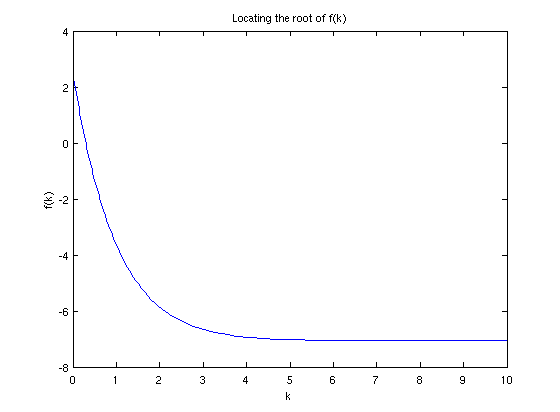
\includegraphics[scale=0.6]{kfunct.png}
\end{center}
\end{figure}

\subsection{T(t)}
\label{troot}
\begin{figure}[H]
\begin{center}
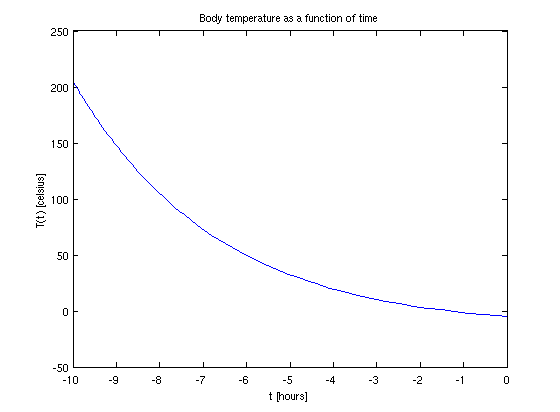
\includegraphics[scale=0.6]{tfunct.png}
\end{center}
\end{figure}

\newpage

\section{Appendix: C}
\label{appc}
\subsection{Error quotient, bisection method}
\label{qbisect}
\begin{figure}[H]
\begin{center}
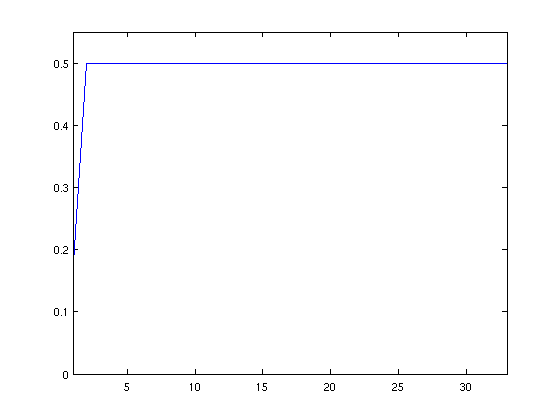
\includegraphics[scale=0.6]{bisect-err-q.png}
\end{center}
\end{figure}

\subsection{Error quotient, secant root method}
 \label{qsecant}
 \begin{figure}[H]
 \begin{center}
 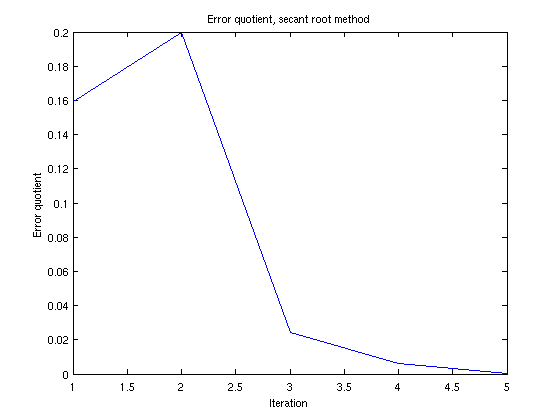
\includegraphics[scale=0.6]{secant-err-q.png}
 \end{center}
 \end{figure}

\subsection{Error quotient, fixed point iteration method}
  \label{qfixedpoint}
  \begin{figure}[H]
  \begin{center}
  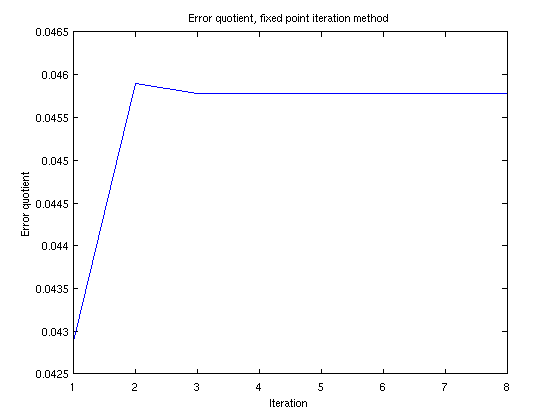
\includegraphics[scale=0.6]{fixed-err-q.png}
  \end{center}
   \end{figure}

\subsection{Error quotient, Newton-Raphson's method}
   \label{qnewton}
   \begin{figure}[H]
   \begin{center}
   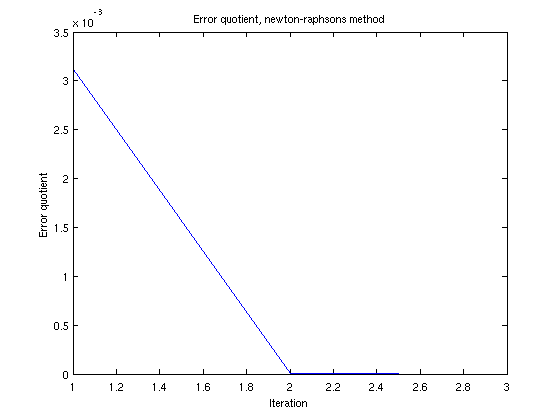
\includegraphics[scale=0.6]{newton-err-q.png}
   \end{center}
   \end{figure}


\end{document}